\documentclass[tikz,border=4pt]{standalone}
\usepackage[T1]{fontenc}
\usepackage{newtxtext}
\usetikzlibrary{arrows.meta,positioning,fit,backgrounds}

\definecolor{commonblue}{HTML}{DCEAF7}
\definecolor{densitygreen}{HTML}{E3F0E5}
\definecolor{pipelineorange}{HTML}{F8E6D2}
\definecolor{ink}{HTML}{263746}
\definecolor{lineblue}{HTML}{427AA1}
\definecolor{linegreen}{HTML}{4F8A5B}
\definecolor{lineorange}{HTML}{C8782D}

\begin{document}
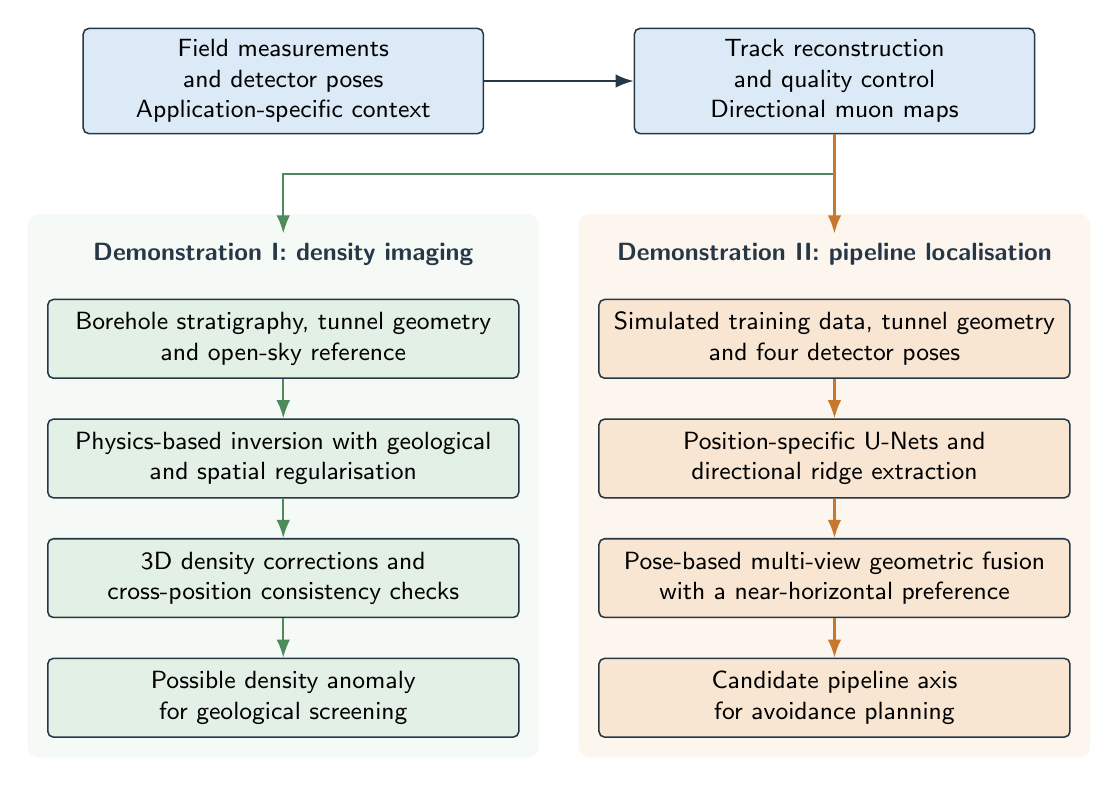
\begin{tikzpicture}[
  font=\sffamily\small,
  >=Latex,
  box/.style={draw=ink, rounded corners=2pt, line width=0.55pt,
    align=center, minimum height=10mm, inner sep=4pt},
  common/.style={box, fill=commonblue, text width=48mm},
  density/.style={box, fill=densitygreen, text width=57mm},
  pipeline/.style={box, fill=pipelineorange, text width=57mm},
  arrow/.style={-{Latex[length=2.3mm]}, line width=0.75pt, draw=ink},
  label/.style={font=\sffamily\bfseries\small, text=ink}
]

\node[common] (acquire) at (-35mm,0)
  {Field measurements and detector poses\\Application-specific context};
\node[common] (maps) at (35mm,0)
  {Track reconstruction and quality control\\Directional muon maps};
\draw[arrow] (acquire) -- (maps);

\node[label] (dlabel) at (-35mm,-22mm)
  {Demonstration I: density imaging};
\node[label] (plabel) at (35mm,-22mm)
  {Demonstration II: pipeline localisation};

\node[density, below=3mm of dlabel] (dinput)
  {Borehole stratigraphy, tunnel geometry\\and open-sky reference};
\node[density, below=5mm of dinput] (dinvert)
  {Physics-based inversion with geological\\and spatial regularisation};
\node[density, below=5mm of dinvert] (dout)
  {3D density corrections and\\cross-position consistency checks};
\node[density, below=5mm of dout] (ddecision)
  {Possible density anomaly\\for geological screening};

\node[pipeline, below=3mm of plabel] (pinput)
  {Simulated training data, tunnel geometry\\and four detector poses};
\node[pipeline, below=5mm of pinput] (pdetect)
  {Position-specific U-Nets and\\directional ridge extraction};
\node[pipeline, below=5mm of pdetect] (pfuse)
  {Pose-based multi-view geometric fusion\\with a near-horizontal preference};
\node[pipeline, below=5mm of pfuse] (pdecision)
  {Candidate pipeline axis\\for avoidance planning};

\draw[arrow, draw=linegreen] (maps.south) -- ++(0,-5mm) -| (dlabel.north);
\draw[arrow, draw=lineorange] (maps.south) -- ++(0,-5mm) -| (plabel.north);
\draw[arrow, draw=linegreen] (dinput) -- (dinvert);
\draw[arrow, draw=linegreen] (dinvert) -- (dout);
\draw[arrow, draw=linegreen] (dout) -- (ddecision);
\draw[arrow, draw=lineorange] (pinput) -- (pdetect);
\draw[arrow, draw=lineorange] (pdetect) -- (pfuse);
\draw[arrow, draw=lineorange] (pfuse) -- (pdecision);

\begin{scope}[on background layer]
  \node[fit=(plabel)(pinput)(pdecision), fill=pipelineorange!35, rounded corners=4pt,
    inner sep=7pt] {};
  \node[fit=(dlabel)(dinput)(ddecision), fill=densitygreen!35, rounded corners=4pt,
    inner sep=7pt] {};
\end{scope}

\end{tikzpicture}
\end{document}